\chapter{Resultados e produtos obtidos}

\section{Implementações concorrentes dos métodos Runge-Kutta, Nearest Neighbour e Interpolação Trilinear}
  \subsection{Protótipo básico}
  O protótipo básico foi uma prova de conceito bem sucedida para a implementação do método implementação em si e suas limitações, bem como para o uso das linguagens CUDA e OpenCL para este fim.
  
  Sua compilação é bastante simples através do comando \textit{make}. Sem nenhum argumento ele compilará a versão em \textit{C++} por padrão. Com os argumentos \textit{cuda} ou \textit{opencl} serão compiladas suas respectivas versões. Abaixo está o processo de compilação
  
  {\scriptsize
  \begin{verbatim}
rafael@BURN-E:~/workspace/runge-kutta$ make cuda
g++ -c -Wall -pedantic -Wextra  -Iinclude main.cpp
g++ -c -Wall -pedantic -Wextra  -Iinclude io/input.cpp
g++ -c -Wall -pedantic -Wextra  -Iinclude core/dataset.cpp
g++ -c -Wall -pedantic -Wextra  -Iinclude core/fiber.cpp
g++ -c -Wall -pedantic -Wextra  -Iinclude io/output.cpp
g++ -c -Wall -pedantic -Wextra  -Iinclude io/gui/primitives/cylinder.cpp
g++ -c -Wall -pedantic -Iinclude io/gui/window_manager.cpp
g++ -c -Wall -pedantic -Wextra  -Iinclude io/gui/scene.cpp
g++ -c -Wall -pedantic -Wextra  -Iinclude io/gui/primitives/cylinder_collection.cpp
g++ -c -Wall -pedantic -Wextra  -Iinclude io/gui/primitives/cone.cpp
g++ -c -Wall -pedantic -Wextra  -Iinclude io/gui/primitives/cone_collection.cpp
nvcc -c -Iinclude core/cuda/rk.cpp -o rk_cuda.o -arch sm_20
nvcc -c -Iinclude core/cuda/rk_kernel.cu -o rk_cuda_kernel.o -arch sm_20
nvcc main.o input.o dataset.o fiber.o output.o cylinder.o window_manager.o scene.o
  cylinder_collection.o cone.o cone_collection.o rk_cuda.o rk_cuda_kernel.o -o rk
  -arch sm_20 -lglut -lGL -lGLU -lm -lpthread -lX11
  \end{verbatim}
  }
  
  \newpage
  Sua interface é bastante básica, mas permite rotacionar o campo e a fibra, translada-lo, aproximá-lo ou afasta-lo tudo através de teclas. Além disso, é possível escolher quais informações são exibidas. Ou seja, é possível escolher entre exibir ou ocultar o campo vetorial, as fibras resultantes do RK2 ou as fibras resultantes do RK4.
  
  A única limitação encontrada para esta implementação é lidar com a inderteminação que existe no campo vetorial na região de intersecção de duas fibras. Esta indeterminação faz com que o método possa seguir qualquer uma das fibras na intersecção quando chega a esta região.
  
  \begin{figure}[!h]
    \begin{center}
      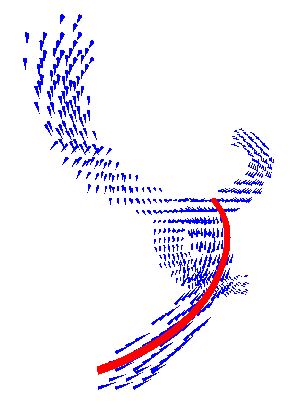
\includegraphics[width=140mm, height=80mm]{images/fibraecampo.png}
      \label{fig:}
      \caption{Campo 32x32x32 com duas hélices. Ao chegar na intersecção, a fibra se desvia para um fora do campo e o método entende que terminou de propaga-la devido à baixa intensidade dos vetores.}
    \end{center}
  \end{figure}
  
  \newpage
  \subsection{Protótipo utilizando a VTK}
\section{Integração com o MedSquare}
